\chapter{Давление, свободная энергия и флуктуации энергии}

\lectureoverview{Мы выводим давление из статистической суммы, не предполагая кинетической картины ударов молекул о стенку. Геометрическая лемма преобразует адиабатическую производную в производные при фиксированной температуре, свободная энергия Гельмгольца дает связь с \(\log Z\), а первым приложением оказывается закон идеального газа. Затем мы используем ту же статистическую сумму, чтобы вывести равновесную флуктуацию энергии и ее связь с теплоемкостью.}

\section{Пусть математика проверит интуицию}

У термодинамики своеобразная репутация. Ее дифференциальное исчисление элементарно, однако выбор того, что дифференцировать и что держать фиксированным, может быть удивительно тонким. Наша задача намеренно узка: вычислить давление идеального газа. Однако путь к этому ответу должен быть достаточно общим и для систем, в которых привычная молекулярная картина уже не заслуживает доверия.

Кинетическую историю рассказать легко. Молекулы ударяются о стенку и меняют знак нормальной компоненты своего импульса. Импульс, переданный за единицу времени, дает силу, а сила на единицу площади дает давление. Мы уже знаем, что средняя кинетическая энергия одной молекулы в трех измерениях равна
\begin{equation}
 \left\langle \frac{p^2}{2m}\right\rangle=\frac{3}{2}T
 \qquad (k_B=1).
 \label{eq:sm5-mean-kinetic-energy}
\end{equation}
При изотропном распределении скоростей можно оценить частоту столкновений, перенос импульса в каждом столкновении и возникающее давление.

Но сама стенка, по-видимому, нарушает изотропию. Почему у молекул очень близко к границе должно быть то же распределение по модулям скоростей и направлениям, что и у молекул глубоко в объеме? В равновесии это так с точностью, существенной здесь, но такой вывод должен следовать из статистической механики, а не незаметно вноситься в расчет в виде интуиции. Столкновения между молекулами делают кинетический аргумент еще менее прозрачным. Невзаимодействующий газ прост именно потому, что это необычно простая система.

В физике бывают случаи, когда самый безопасный прием — временно отказаться от наглядной картины и положиться на математику. Сначала выделяют искомую величину, затем преобразуют общие соотношения и ждут, пока не появится узнаваемая формула. В конце интуиция возвращается, но тогда математика проверяет интуицию, а не наоборот. Удовольствие термодинамики состоит в удивительных соотношениях, которые возникают из этой процедуры.

Искомое соотношение — это уравнение состояния,
\begin{equation}
 P=P(T,V,N),
 \label{eq:sm5-equation-of-state-target}
\end{equation}
где \(N\) — количество вещества, \(T\) — температура, а \(V\) — объем. Удовлетворительный вывод должен по-прежнему иметь смысл, когда частицы взаимодействуют, или когда вещество является жидкостью, плазмой или твердым телом. Только окончательное вычисление статистической суммы будет специфично для идеального газа.

\section{Энтропия и свободная энергия Гельмгольца}

Для начала напомним канонические формулы, которые понадобятся позже. Для микросостояний, помеченных \(i\),
\begin{equation}
 \begin{aligned}
 S&=-\sum_i p_i\log p_i,\\
 p_i&=\frac{e^{-\beta E_i}}{Z},\\
 Z&=\sum_i e^{-\beta E_i}.
 \end{aligned}
 \label{eq:sm5-canonical-definitions}
\end{equation}
Логарифм вероятности равен
\begin{equation}
 \log p_i=-\beta E_i-\log Z.
 \label{eq:sm5-log-probability}
\end{equation}
Подстановка в выражение для энтропии дает
\begin{align}
 S
 &=-\sum_i p_i\log p_i \notag\\
 &=\beta\sum_i p_iE_i+\log Z\sum_i p_i \notag\\
 &=\beta E+\log Z.
 \label{eq:sm5-entropy-log-z}
\end{align}
Здесь \(E=\sum_i p_iE_i\) — средняя энергия.

\begin{classroomqa}
\audiencequestion{Почему второй член дает только \(\log Z\), а не число состояний, умноженное на \(\log Z\)?}
\lecturerresponse{Суммируемый коэффициент — \(p_i\), а не \(1\). Нормировка дает \(\sum_i p_i=1\). Эквивалентно, числитель \(\sum_i e^{-\beta E_i}=Z\) сокращает \(Z\) в знаменателе. Число состояний на этом шаге вообще не появляется.
\lecturetimestamp{00:14:25--00:14:55}}
\end{classroomqa}

В энергетических единицах, используемых на большей части лекции, \(\beta=1/T\). Умножая \eqref{eq:sm5-entropy-log-z} на \(T\) и перегруппировывая члены, получаем
\begin{equation}
 E-TS=-T\log Z.
 \label{eq:sm5-helmholtz-identity}
\end{equation}
Комбинация в левой части встречается настолько часто, что заслуживает отдельного имени:
\begin{equation}
 A\equiv E-TS,
 \qquad
 A=-T\log Z.
 \label{eq:sm5-helmholtz-definition}
\end{equation}
Это свободная энергия Гельмгольца. Сейчас важнее не название, а само тождество; оно понадобится нам, когда давление будет преобразовано в производную статистической суммы.

\begin{figure}[t]
\centering
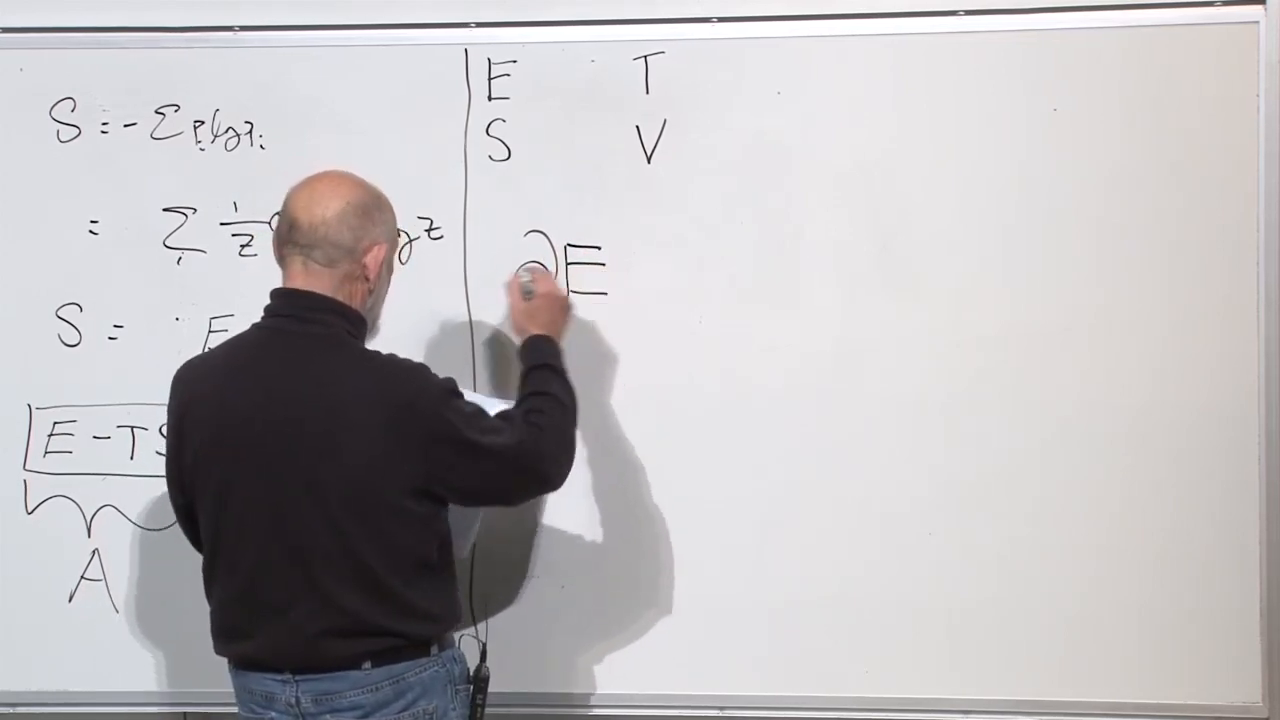
\includegraphics[width=0.90\textwidth]{lecture_05_figure_03.png}
\caption{Каноническое соотношение для энтропии, переписанное в виде \(A=E-TS=-T\log Z\).}
\lectureframe{00:16:50}
\end{figure}

\section{Управляющие параметры и их отклики}

Управляющий параметр — это макроскопическая величина, которую экспериментатор может изменять извне. Перемещая поршень, мы меняем объем, не манипулируя отдельными молекулами. Другими примерами служат приложенные электрические и магнитные поля. В более общем ансамбле можно также допустить изменение числа частиц.

Термодинамические переменные естественным образом образуют сопряженные пары. В данной задаче управляющим параметром является объем, а откликом на него — давление. Мы изменяем \(V\); давление показывает, как система энергетически сопротивляется этому изменению. Позже производная энергии сделает эту сопряженность точной.

\begin{classroomqa}
\audiencequestion{Можно ли само давление рассматривать как управляющий параметр?}
\lecturerresponse{Можно поставить эксперимент, в котором фиксируется внешнее давление, но в используемой здесь постановке положение поршня фиксирует объем, а внутреннее давление является откликом. Давление и объем — сопряженные переменные; какая из этих величин управляется, зависит от ансамбля и экспериментальной установки.
\lecturetimestamp{00:19:22--00:20:01}}
\end{classroomqa}

\begin{classroomqa}
\audiencequestion{Предполагается ли, что все молекулы одинаковы, или рассуждение ограничено газом?}
\lecturerresponse{Нет, такое ограничение не требуется для термодинамического рассуждения. Цилиндр может содержать несколько видов частиц, жидкость или даже твердое тело, подвергаемое сжатию. Статистическая сумма идеального газа будет лишь частным применением после того, как установлена общая формула для давления.
\lecturetimestamp{00:20:02--00:20:39}}
\end{classroomqa}

\begin{classroomqa}
\audiencequestion{Можно ли изменять количество вещества как еще одно внешнее воздействие?}
\lecturerresponse{Да. Число частиц — еще один возможный управляющий параметр. Если рассматривать его как динамическую величину, возникает собственная сопряженная переменная — химический потенциал. Для сегодняшнего вычисления \(N\) остается фиксированным.
\lecturetimestamp{00:20:39--00:20:57}}
\end{classroomqa}

\begin{classroomqa}
\audiencequestion{Могут ли жидкая вода и водяной пар одновременно присутствовать в равновесии?}
\lecturerresponse{При температуре и давлении сосуществования — да. Гравитация может располагать жидкость ниже пара, и все же обе фазы могут иметь одну и ту же температуру и оставаться в тепловом равновесии. Применима та же общая статистико-механическая схема.
\lecturetimestamp{00:20:59--00:21:36}}
\end{classroomqa}

В следующем рассуждении рассматривайте энергию и энтропию как зависимые функции двух независимо регулируемых переменных:
\begin{equation}
 E=E(T,V),
 \qquad
 S=S(T,V).
 \label{eq:sm5-dependent-functions}
\end{equation}
Температура и объем задают координаты в термодинамическом пространстве состояний. Энергия и энтропия ставят в соответствие числа каждой равновесной точке этого пространства.

\section{Производная при постоянной энтропии}

Производная, которая нам в конечном счете нужна, необычна:
\[
 \left(\frac{\partial E}{\partial V}\right)_S.
\]
Хотя \(T\) и \(V\) являются независимыми координатами, эта производная требует изменять \(V\), одновременно накладывая условие, что зависимая функция \(S(T,V)\) остается постоянной. Это производная вдоль кривой на плоскости \((T,V)\), а не вдоль координатной оси.

\begin{classroomqa}
\audiencequestion{Как \(T\) и \(V\) могут быть независимыми, если позднее используется производная \(dT/dV\)?}
\lecturerresponse{Они независимы на всем пространстве состояний. Как только мы накладываем ограничение \(S(T,V)=\mathrm{constant}\), допустимые состояния лежат на одномерном контуре. Вдоль этого контура \(T\) становится функцией \(V\), и его наклон \(dT/dV\) определен однозначно.
\lecturetimestamp{01:01:18--01:02:09}}
\end{classroomqa}

\begin{lemma}
Если \(E(T,V)\) и \(S(T,V)\) дифференцируемы, то везде, где
\((\partial S/\partial T)_V\neq0\),
\begin{equation}
 \left(\frac{\partial E}{\partial V}\right)_S
 =
 \left(\frac{\partial E}{\partial V}\right)_T
 -
 \left(\frac{\partial E}{\partial S}\right)_V
 \left(\frac{\partial S}{\partial V}\right)_T.
 \label{eq:sm5-calculus-lemma}
\end{equation}
\end{lemma}

\begin{proof}
Для произвольного бесконечно малого смещения,
\begin{equation}
 dE=
 \left(\frac{\partial E}{\partial V}\right)_T dV
 +
 \left(\frac{\partial E}{\partial T}\right)_V dT.
 \label{eq:sm5-total-differential-e}
\end{equation}
При фиксированном \(V\) правило цепочки позволяет использовать \(S\) как промежуточную переменную:
\begin{equation}
 \left(\frac{\partial E}{\partial T}\right)_V
 =
 \left(\frac{\partial E}{\partial S}\right)_V
 \left(\frac{\partial S}{\partial T}\right)_V.
 \label{eq:sm5-chain-rule-e-s-t}
\end{equation}

Теперь ограничим смещение контуром, на котором \(S\) постоянно. Вдоль этого контура,
\begin{equation}
 0=dS=
 \left(\frac{\partial S}{\partial V}\right)_T dV
 +
 \left(\frac{\partial S}{\partial T}\right)_V dT.
 \label{eq:sm5-constant-entropy-differential}
\end{equation}
Решая относительно наклона контура, получаем
\begin{equation}
 \left(\frac{dT}{dV}\right)_S
 =
 -
 \frac{\left(\frac{\partial S}{\partial V}\right)_T}
 {\left(\frac{\partial S}{\partial T}\right)_V}.
 \label{eq:sm5-entropy-contour-slope}
\end{equation}
Разделим \eqref{eq:sm5-total-differential-e} на \(dV\), воспользуемся
\eqref{eq:sm5-chain-rule-e-s-t}
и подставим
\eqref{eq:sm5-entropy-contour-slope}:
\begin{align}
 \left(\frac{\partial E}{\partial V}\right)_S
 &=
 \left(\frac{\partial E}{\partial V}\right)_T
 +
 \left(\frac{\partial E}{\partial S}\right)_V
 \left(\frac{\partial S}{\partial T}\right)_V
 \left(\frac{dT}{dV}\right)_S \notag\\
 &=
 \left(\frac{\partial E}{\partial V}\right)_T
 -
 \left(\frac{\partial E}{\partial S}\right)_V
 \left(\frac{\partial S}{\partial V}\right)_T.
\end{align}
Множитель \((\partial S/\partial T)_V\) сократился, что и доказывает результат.
\end{proof}

\begin{figure}[t]
\centering
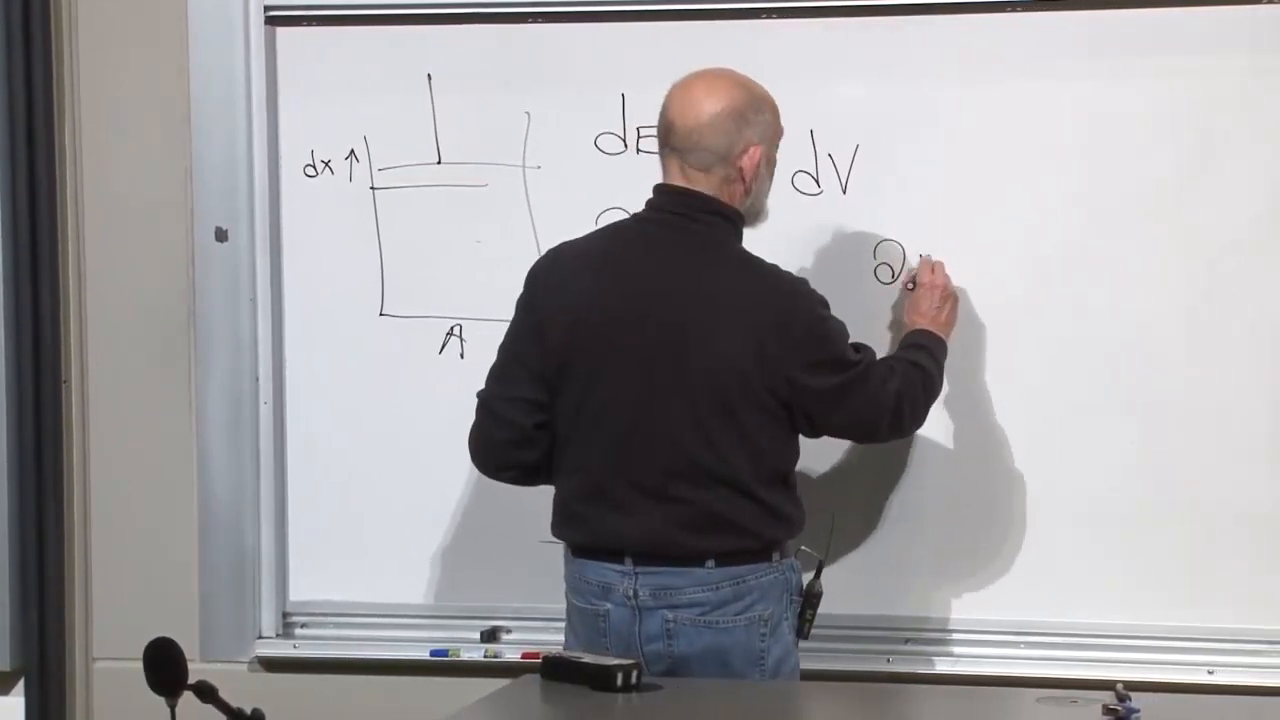
\includegraphics[width=0.90\textwidth]{lecture_05_figure_04.png}
\caption{Вычисление вдоль контура постоянной энтропии на этапе сокращения, завершающего лемму о производной.}
\lectureframe{00:36:10}
\end{figure}

Геометрическая картина здесь не просто украшение. Она объясняет, почему кажущаяся странной производная при фиксированном \(S\) может быть вычислена с помощью обычных частных производных по независимым координатам \(T\) и \(V\). Запись \(\delta E/\delta V\) в ходе построения служит полезным напоминанием о том, что эти символы представляют собой отношения малых изменений вдоль заданного пути.

\begin{classroomqa}
\audiencequestion{Является ли разложение \(dE\) просто обычным определением частных производных?}
\lecturerresponse{Да. В полном дифференциале ничего особенного не происходит. Единственная дополнительная деталь — последующее ограничение на контур \(dS=0\), которое определяет связь между \(dT\) и \(dV\).
\lecturetimestamp{00:29:26--00:29:32}}
\end{classroomqa}

\begin{classroomqa}
\audiencequestion{Требуется ли для сокращения, чтобы
\((\partial S/\partial T)_V\) была ненулевой?}
\lecturerresponse{Да. Для обычной устойчивой системы,
\[
 \left(\frac{\partial S}{\partial T}\right)_V
 =\frac{C_V}{T}>0,
\]

так что деление допустимо. Исключительные точки требуют отдельного рассмотрения.
При фиксированном гамильтониане повышение температуры расширяет каноническое распределение энергии и обычно увеличивает энтропию; понижение температуры сужает его. Именно таково физически правильное направление аргумента о монотонности.
\lecturetimestamp{00:36:50--00:37:47}}
\end{classroomqa}

\section{Работа поршня и адиабатическое условие}

Теперь придадим производной физический смысл. Рассмотрим поршень с
площадью поперечного сечения \(\mathcal A\). Если он смещается наружу на \(dx\), то
\begin{equation}
 dV=\mathcal A\,dx.
 \label{eq:sm5-piston-volume}
\end{equation}
Газ действует на поршень силой \(P\mathcal A\), поэтому работа,
совершаемая газом, равна
\begin{equation}
 \delta W_{\mathrm{by}}=P\mathcal A\,dx=P\,dV.
 \label{eq:sm5-piston-work}
\end{equation}
Если тепло в газ не поступает, то из закона сохранения энергии следует
\begin{equation}
 dE=-P\,dV.
 \label{eq:sm5-adiabatic-work}
\end{equation}
Знак имеет физический смысл: при расширении газ поднимает поршень или сообщает ему ускорение, а его собственная энергия уменьшается.

\begin{figure}[t]
\centering
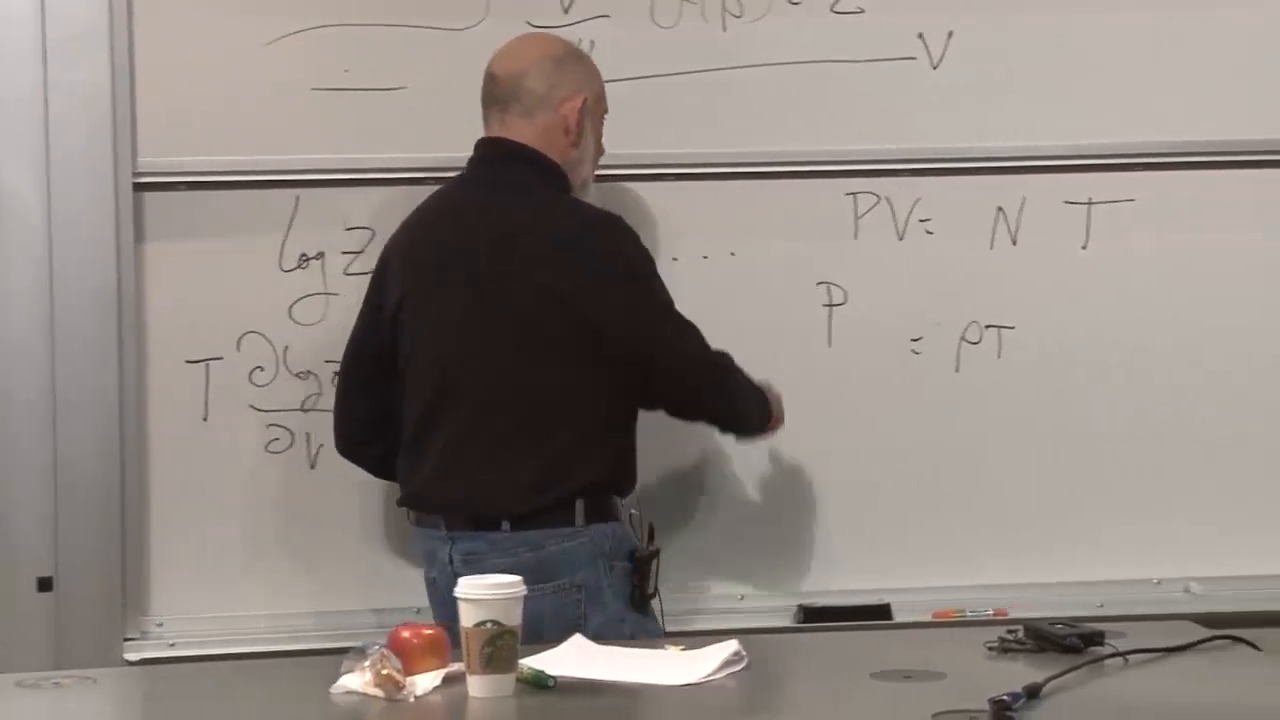
\includegraphics[width=0.90\textwidth]{lecture_05_figure_05.png}
\caption{Геометрия поршня и полученное соотношение для работы
\(dE=-P\,dV\).}
\lectureframe{00:43:10}
\end{figure}

Существенны две оговорки. Поршень должен двигаться достаточно медленно,
чтобы система оставалась сколь угодно близкой к равновесию, а стенки должны быть
теплоизолированы, чтобы энергия не подводилась в виде тепла. Быстрое вытягивание может быть настолько
стремительным, что за время движения ни одна молекула не достигнет удаляющегося поршня. Быстрое
сжатие порождает ударные волны. Ни один из этих процессов не представим
последовательностью равновесных состояний.

Термин \emph{адиабатический} иногда означает отсутствие теплообмена, а
иногда — медленное изменение. В обратимом процессе, который здесь требуется, присутствуют
обе идеи: изменение квазистатично и система теплоизолирована. При этих
условиях процесс также изоэнтропичен.

\begin{classroomqa}
\audiencequestion{Почему при адиабатическом изменении энтропия остается постоянной?}
\lecturerresponse{Рассмотрим систему с квантово-механической точки зрения. Ее многочастичные
энергетические уровни зависят от объема. Когда \(V\) медленно изменяется, адиабатическая
теорема непрерывно переводит каждый занятый уровень в его продолжение без
переходов между метками уровней. Энергии \(E_i(V)\) изменяются, но
вероятности заселения \(p_i\) остаются фиксированными. Поскольку
\(S=-\sum_i p_i\log p_i\) зависит от этих вероятностей, энтропия остается
постоянной. Теплообмен или необратимое движение сделали бы этот
вывод недействительным.
\lecturetimestamp{00:43:37--00:49:15}}
\end{classroomqa}

\begin{figure}[t]
\centering
\includegraphics[width=0.90\textwidth]{lecture_05_figure_06.png}
\caption{Многочастичные энергетические уровни, изменяющиеся с объемом, тогда как
вероятности их заселения сохраняют привязку к меткам уровней.}
\lectureframe{00:48:50}
\end{figure}

Уравнение \eqref{eq:sm5-adiabatic-work}, рассмотренное вдоль этого пути с постоянной
энтропией, задает давление в виде
\begin{equation}
 P=-\left(\frac{\partial E}{\partial V}\right)_S.
 \label{eq:sm5-pressure-fixed-entropy}
\end{equation}
Это сопряженное соотношение между давлением и объемом.

\begin{classroomqa}
\audiencequestion{Что происходит, если вместо этого перемещать поршень быстро?}
\lecturerresponse{Система выходит из равновесия, и детали ее динамики
становятся существенными. Внезапное сжатие порождает ударную волну.
При идеальном свободном расширении поршень может удалиться прежде, чем в него ударится хоть одна молекула, так что работа не совершается и
энергия остается постоянной, хотя объем меняется. Позднее газ
релаксирует к равновесию с возросшей энтропией. Такие процессы нельзя
описать единственной равновесной производной в
\eqref{eq:sm5-pressure-fixed-entropy}.
\lecturetimestamp{00:58:30--01:01:15}}
\end{classroomqa}

\begin{classroomqa}
\audiencequestion{Какое количественное условие определяет, является ли изменение
медленным?}
\lecturerresponse{Характерное время внешнего изменения должно быть велико по сравнению с
соответствующими внутренними временами релаксации. Для газа во время
макроскопического изменения должно происходить много молекулярных
столкновений и много ударов о стенки. Точный масштаб времени зависит от
вещества и геометрии, тогда как сам квазистатический предел является общим.
\lecturetimestamp{01:02:09--01:03:20}}
\end{classroomqa}

\section{От адиабатической энергии к статистической сумме}

Физическая формула \eqref{eq:sm5-pressure-fixed-entropy} пока еще не самая
удобная для вычисления. Каноническая статистическая механика естественным образом дает
функции температуры, потому что \(T\) непосредственно входит в больцмановский
вес. Лемма анализа переводит неудобную производную при фиксированной
энтропии в удобный для вычислений язык:
\begin{align}
 P
 &=
 -\left(\frac{\partial E}{\partial V}\right)_T
 +
 \left(\frac{\partial E}{\partial S}\right)_V
 \left(\frac{\partial S}{\partial V}\right)_T.
 \label{eq:sm5-pressure-lemma-substitution}
\end{align}
При фиксированном объеме первое начало дает \(dE=T\,dS\), и потому
\begin{equation}
 \left(\frac{\partial E}{\partial S}\right)_V=T.
 \label{eq:sm5-e-s-temperature}
\end{equation}
Следовательно
\begin{equation}
 P=
 -\left(\frac{\partial E}{\partial V}\right)_T
 +
 T\left(\frac{\partial S}{\partial V}\right)_T.
 \label{eq:sm5-pressure-fixed-temperature-pieces}
\end{equation}

\begin{classroomqa}
\audiencequestion{Откуда берется знак минус в формуле для давления?}
\lecturerresponse{Он возникает из работы, совершаемой газом:
\(dE=-P\,dV\) при адиабатическом расширении. В самой лемме анализа между ее
двумя членами стоит минус; общий минус в
\(P=-(\partial E/\partial V)_S\) меняет знак у них обоих, давая
\eqref{eq:sm5-pressure-fixed-temperature-pieces}.
\lecturetimestamp{00:52:40--00:53:14}}
\end{classroomqa}

Поскольку \(T\) фиксирована в обеих производных,
\begin{align}
 P
 &=
 -\left(\frac{\partial}{\partial V}(E-TS)\right)_T \notag\\
 &=
 -\left(\frac{\partial A}{\partial V}\right)_T.
 \label{eq:sm5-pressure-free-energy}
\end{align}
Наконец, подставим \(A=-T\log Z\):
\begin{equation}
 \boxed{
 P=
 T\left(\frac{\partial\log Z}{\partial V}\right)_T
 }.
 \label{eq:sm5-pressure-log-z}
\end{equation}

\begin{figure}[t]
\centering
\includegraphics[width=0.90\textwidth]{lecture_05_figure_07.png}
\caption{Сведение рассуждения при фиксированной температуре:
\(P=-(\partial A/\partial V)_T
=T(\partial\log Z/\partial V)_T\).}
\lectureframe{00:55:55}
\end{figure}

В \eqref{eq:sm5-pressure-log-z} нигде не предполагается идеальный газ. Если статистическую
сумму можно вычислить для взаимодействующей жидкости, плазмы или
твердого тела, то та же производная дает соответствующее давление. В более общем
виде каждому внешнему управляющему параметру соответствует сопряженный
отклик, получаемый дифференцированием подходящего термодинамического потенциала. В статистической
сумме закодированы многие такие отклики: дифференцирование \(\log Z\) по
\(\beta\) дает энергию, тогда как дифференцирование по
объему дает давление.

\section{Уравнение состояния идеального газа}

Лишь теперь перейдем к случаю \(N\) невзаимодействующих частиц. При сохранении классической
нормировки фазового пространства
\begin{equation}
 Z_N=
 \frac{1}{N!h^{3N}}
 \int d^{3N}q\,d^{3N}p\,
 \exp\!\left[
 -\beta\sum_{a=1}^{N}\frac{\mathbf p_a^2}{2m}
 \right].
 \label{eq:sm5-ideal-gas-partition-integral}
\end{equation}
Имеется \(3N\) координат положения и \(3N\) компонент импульса. Гамильтониан
не зависит от координат, поэтому каждая частица дает один множитель
объема сосуда:
\begin{equation}
 Z_N=
 \frac{V^N}{N!h^{3N}}I_p(\beta),
 \label{eq:sm5-ideal-gas-factorization}
\end{equation}
где весь интеграл по импульсам \(I_p(\beta)\) не зависит от \(V\).

\begin{classroomqa}
\audiencequestion{Почему здесь \(3N\) интегралов по координатам и \(3N\)
интегралов по импульсам?}
\lecturerresponse{Каждая из \(N\) частиц имеет три пространственные координаты
и три сопряженные компоненты импульса. Подсчет дает \(3N\) в каждой половине
фазового пространства, а не \(N\) частиц плюс еще \(3N\) частиц.
\lecturetimestamp{01:04:19--01:04:28}}
\end{classroomqa}

Логарифмирование отделяет зависимость от объема:
\begin{equation}
 \log Z_N
 =
 N\log V-\log N!-3N\log h+\log I_p(\beta).
 \label{eq:sm5-log-ideal-gas-partition}
\end{equation}
Множители \(1/N!\), \(h^{-3N}\) и \(I_p(\beta)\) все не зависят от
объема. Они важны для абсолютной энтропии и других вопросов, но не для
этой конкретной производной. Поэтому
\begin{equation}
 \left(\frac{\partial\log Z_N}{\partial V}\right)_T
 =\frac{N}{V}.
 \label{eq:sm5-log-z-volume-derivative}
\end{equation}
Уравнение \eqref{eq:sm5-pressure-log-z} сразу дает
\begin{equation}
 P=\frac{NT}{V},
 \qquad
 \boxed{PV=NT}.
 \label{eq:sm5-ideal-gas-law}
\end{equation}

\begin{classroomqa}
\audiencequestion{Означает ли \(N\) по-прежнему число реплик, использованных при выводе
распределения Больцмана?}
\lecturerresponse{Нет. Конструкция с репликами в предыдущем выводе была лишь счетным приемом и
здесь уже отсутствует. Здесь \(N\) — это число
реальных частиц в этом одном образце газа.
\lecturetimestamp{01:07:38--01:08:05}}
\end{classroomqa}

Введя численную плотность
\begin{equation}
 \rho=\frac{N}{V}
 \label{eq:sm5-number-density}
\end{equation}
получаем эквивалентную форму
\begin{equation}
 P=\rho T.
 \label{eq:sm5-density-equation-of-state}
\end{equation}

\begin{classroomqa}
\audiencequestion{Следует ли получать форму через плотность делением на \(N\)
или на \(V\)?}
\lecturerresponse{Разделите \(PV=NT\) на \(V\):
\(P=(N/V)T=\rho T\). Здесь \(\rho\) — численная плотность, а не массовая плотность.
\lecturetimestamp{01:08:45--01:09:16}}
\end{classroomqa}

\begin{figure}[t]
\centering
\includegraphics[width=0.90\textwidth]{lecture_05_figure_08.png}
\caption{Производная \(\log Z\) по объему и получающееся из нее уравнение состояния
идеального газа \(PV=NT\), или \(P=\rho T\).}
\lectureframe{01:09:25}
\end{figure}

Возвращаясь к лабораторной температуре \(T_K\),
\begin{equation}
 PV=Nk_BT_K.
 \label{eq:sm5-ideal-gas-law-laboratory}
\end{equation}
Этот знакомый результат согласуется с кинетической интуицией, но его вывод теперь
опирается на формализм, применимый далеко за пределами свободного газа.

\section{Второй выигрыш: равновесные флуктуации}

Вычисление давления завершено, но остается один обещанный вопрос:
что еще можно извлечь из статистической суммы? Рассмотрим систему,
находящуюся в тепловом контакте с термостатом. Ее энергия не фиксирована.
Энергия поступает и уходит, поэтому результаты повторных измерений флуктуируют вокруг канонического среднего.

\begin{classroomqa}
\audiencequestion{Можем ли мы теперь вычислить обещанные флуктуации?}
\lecturerresponse{Да. Оставшееся время позволяет еще раз продемонстрировать тот
же принцип: производные \(Z\) кодируют измеримую термодинамическую
информацию.
\lecturetimestamp{01:10:37--01:10:50}}
\end{classroomqa}

\subsection{Дисперсия и стандартное отклонение}

Для случайной величины \(x\) с \(\langle x\rangle=0\) мерой
ширины распределения служит \(\langle x^2\rangle\). Для общего распределения
сдвинем переменную на ее среднее:
\begin{equation}
 \delta x=x-\langle x\rangle.
 \label{eq:sm5-centered-variable}
\end{equation}
Ее среднее равно нулю,
\begin{equation}
 \langle\delta x\rangle
 =
 \langle x\rangle-\langle x\rangle=0,
 \label{eq:sm5-centered-mean}
\end{equation}
а ее средний квадрат равен
\begin{align}
 (\Delta x)^2
 &\equiv
 \left\langle\left(x-\langle x\rangle\right)^2\right\rangle \notag\\
 &=
 \langle x^2\rangle
 -2\langle x\rangle^2
 +\langle x\rangle^2 \notag\\
 &=
 \langle x^2\rangle-\langle x\rangle^2.
 \label{eq:sm5-variance}
\end{align}
Это и есть дисперсия. Ее положительный квадратный корень \(\Delta x\) — это стандартное
отклонение.

\begin{classroomqa}
\audiencequestion{Почему среднее от
\(x-\langle x\rangle\) в точности равно нулю?}
\lecturerresponse{Усреднение линейно, а \(\langle x\rangle\) уже является
числом. Поэтому
\(\langle x-\langle x\rangle\rangle
=\langle x\rangle-\langle x\rangle=0\).
\lecturetimestamp{01:14:02--01:14:22}}
\end{classroomqa}

\begin{classroomqa}
\audiencequestion{В чем различие между квадратом флуктуации, дисперсией, среднеквадратичной шириной и стандартным отклонением?}
\lecturerresponse{Дисперсия равна
\((\Delta x)^2=\langle x^2\rangle-\langle x\rangle^2\).
Стандартное отклонение — ее квадратный корень, \(\Delta x\). Для переменной с нулевым средним стандартное отклонение также является ее среднеквадратичным значением.
\lecturetimestamp{01:16:39--01:18:38}}
\end{classroomqa}

\begin{figure}[t]
\centering
\includegraphics[width=0.90\textwidth]{lecture_05_figure_09.png}
\caption{Сдвинутая переменная и разложение, приводящее к
\((\Delta x)^2=\langle x^2\rangle-\langle x\rangle^2\).}
\lectureframe{01:17:20}
\end{figure}

\subsection{Моменты энергии из статистической суммы}

Для канонического ансамбля,
\begin{align}
 \langle E\rangle
 &=
 \frac{1}{Z}\sum_i E_i e^{-\beta E_i} \notag\\
 &=
 -\frac{1}{Z}\frac{\partial Z}{\partial\beta}
 =
 -\frac{\partial\log Z}{\partial\beta}.
 \label{eq:sm5-mean-energy-from-z}
\end{align}
Одно дифференцирование по \(\beta\) со знаком минус дает умножение на один множитель \(E_i\). Вторая производная порождает \(E_i^2\):
\begin{equation}
 \langle E^2\rangle
 =
 \frac{1}{Z}\sum_i E_i^2e^{-\beta E_i}
 =
 \frac{1}{Z}\frac{\partial^2 Z}{\partial\beta^2}.
 \label{eq:sm5-second-energy-moment}
\end{equation}
Следовательно, дисперсия энергии равна
\begin{align}
 (\Delta E)^2
 &=
 \langle E^2\rangle-\langle E\rangle^2 \notag\\
 &=
 \frac{1}{Z}\frac{\partial^2Z}{\partial\beta^2}
 -
 \frac{1}{Z^2}
 \left(\frac{\partial Z}{\partial\beta}\right)^2 \notag\\
 &=
 \frac{\partial^2\log Z}{\partial\beta^2}
 =
 -\frac{\partial\langle E\rangle}{\partial\beta}.
 \label{eq:sm5-energy-variance-beta}
\end{align}
И снова на вид сложная наблюдаемая величина оказывается производной от
\(\log Z\).

\begin{figure}[t]
\centering
\includegraphics[width=0.90\textwidth]{lecture_05_figure_10.png}
\caption{Вторая производная \(\log Z\) по \(\beta\), отождествленная с дисперсией энергии.}
\lectureframe{01:29:00}
\end{figure}

\subsection{Теплоемкость и величина флуктуаций}

В используемых на лекции единицах \(T=1/\beta\), поэтому
\begin{equation}
 -\frac{\partial}{\partial\beta}
 =
 T^2\frac{\partial}{\partial T}.
 \label{eq:sm5-beta-temperature-derivative}
\end{equation}
При фиксированном объеме определим теплоемкость всего образца как
\begin{equation}
 C_V\equiv
 \left(\frac{\partial\langle E\rangle}{\partial T}\right)_V.
 \label{eq:sm5-heat-capacity}
\end{equation}
Уравнение \eqref{eq:sm5-energy-variance-beta} принимает вид
\begin{equation}
 \boxed{(\Delta E)^2=T^2C_V}
 \qquad (k_B=1).
 \label{eq:sm5-energy-fluctuation-lecture-units}
\end{equation}
Для лабораторной температуры \(T_K\), где
\(\beta=(k_BT_K)^{-1}\),
\begin{equation}
 \boxed{(\Delta E)^2=k_BT_K^2C_V}.
 \label{eq:sm5-energy-fluctuation-laboratory}
\end{equation}

\begin{figure}[t]
\centering
\includegraphics[width=0.90\textwidth]{lecture_05_figure_11.png}
\caption{Переход от производной по \(\beta\) к теплоемкости при фиксированном объеме, включая восстановленный множитель \(k_B\).}
\lectureframe{01:31:10}
\end{figure}

\begin{classroomqa}
\audiencequestion{Нужно ли в производной указывать фиксированный объем, а не фиксированное давление?}
\lecturerresponse{Да. В этом каноническом выводе внешние управляющие параметры гамильтониана, включая \(V\), удерживаются фиксированными. Получающаяся величина — \(C_V\). Ансамбль при постоянном давлении допускает флуктуации объема и работы и требует соответствующего термодинамического потенциала; нельзя просто заменить \(C_V\) на \(C_P\) в
\eqref{eq:sm5-energy-fluctuation-laboratory}.
\lecturetimestamp{01:29:01--01:29:28; 01:32:50--01:33:21}}
\end{classroomqa}

\begin{classroomqa}
\audiencequestion{Является ли \(C_V\) константой вещества?}
\lecturerresponse{Вообще говоря, нет. Она может зависеть от температуры, объема, фазы и состава. Кроме того, \(C_V\) здесь — теплоемкость всего образца и потому является экстенсивной величиной. Теплоемкость, отнесенную к массе, числу частиц или количеству вещества, получают только после деления на массу, число частиц или количество вещества.
\lecturetimestamp{01:31:47--01:32:21; 01:33:23--01:34:55}}
\end{classroomqa}

Для обычного экстенсивного вещества \(C_V\) пропорциональна \(N\), поэтому
\((\Delta E)^2\) пропорциональна \(N\), а \(\Delta E\) —
\(\sqrt{N}\). Сама средняя энергия пропорциональна \(N\). Следовательно,
\begin{equation}
 \frac{\Delta E}{\langle E\rangle}\sim\frac{1}{\sqrt{N}}.
 \label{eq:sm5-relative-fluctuation-scaling}
\end{equation}
Макроскопические относительные флуктуации ничтожны, тогда как в микроскопических образцах они проявляются непосредственно. Появление \(k_B\) в
\eqref{eq:sm5-energy-fluctuation-laboratory} указывает на эту связь между
термодинамическими наблюдаемыми и молекулярной дискретностью; или, что то же самое, оно связывает макроскопические единицы с подсчетом на авогадровском масштабе.

Давление и флуктуации теперь выводятся из одного и того же объекта:
\[
 P=T\left(\frac{\partial\log Z}{\partial V}\right)_T,
 \qquad
 (\Delta E)^2=\frac{\partial^2\log Z}{\partial\beta^2}.
\]
Это главный вывод. Как только правильно определены ограничения, статистическая сумма не просто нормирует вероятности. Ее производные задают измеримую термодинамику системы.
